\section{漏洞检测}\label{sec:detection}

\begin{figure*}[t]
  \centering
  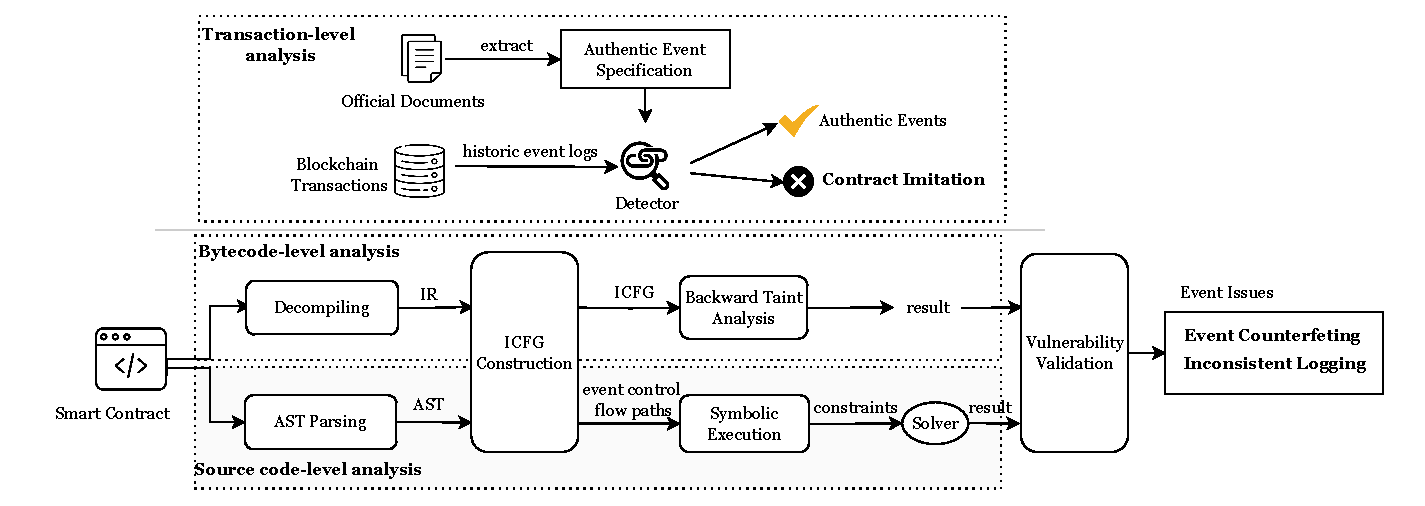
\includegraphics[width=\linewidth]{Sections/Picture/PhatomEventOverview.pdf}
  \caption{\tool 的架构。}
  \label{fig:tool}
\end{figure*}

本节重点讨论与\cref{sec:vector}中攻击向量相关的漏洞检测。我们介绍一种混合方法，该方法结合静态分析、符号执行和链上数据监控，以实现全面的漏洞检测。

\subsection{\tool 框架设计}

如\cref{fig:tool}所示，我们的检测方法采用多层级策略，覆盖交易级、字节码级和源代码级漏洞检测。

在交易级，由于不同项目中的真实事件和发出者存在差异，我们人工研究了不同项目的文档，以建立适当的规则。这些规则被应用于历史和实时链上交易数据，通过识别幻影事件与真实事件混合的实例来检测\emph{合约仿冒}。

对于智能合约，我们的分析同时覆盖字节码和源代码两个层面。首先，我们使用 Gigahorse~\cite{Gigahorse} 将智能合约字节码反编译为三地址形式的中间表示（intermediate representation，IR）。随后，基于该 IR 的基本块构建跨合约控制流图（inter-contract control flow graph，ICFG）。该图支持后向污点分析，我们利用它追踪与事件相关的路径，并检测与\emph{事件仿冒}和\emph{不一致日志记录}相关的漏洞。

如果源代码可用，我们会使用 Slither 扩展分析并执行源代码级分析。通过追踪事件相关调用路径并提取用于符号执行的约束，该分析能够对\emph{事件仿冒}进行二次确认，使我们能够更全面地验证参数值。

由于某些攻击具有特殊性质，\emph{事件处理错误}高度依赖链下系统验证，因此缺乏特定的检测方法。类似地，\emph{转账事件欺骗}主要是一类社会工程学攻击，其分析重点在于代币行为。因此，我们的工具主要针对其余三类攻击进行检测：\emph{事件仿冒}、\emph{不一致日志记录}和\emph{合约仿冒}。这些攻击具有较为明确的模式和合约级漏洞，因而能够被有效识别和处理。

\subsection{交易级检测}
在交易级，我们采用链下监控来分析链上交易数据，并检测潜在的\emph{合约仿冒}攻击。通过基于智能合约预期行为建立领域特定规则，我们系统地验证交易是否符合正确逻辑，并识别任何可能表明幻影事件或未授权交互的恶意活动迹象。

该分析涉及解析交易数据，并应用一组规则来验证事件的关键方面，包括：（1）确保发出的事件具有正确的签名；（2）验证事件发出者是否与预期合约地址匹配；（3）检查函数执行路径是否符合预期逻辑；（4）确认事件参数值是否与预期值一致。

通过执行这些规则，我们能够检测可能表明\emph{合约仿冒}攻击的异常。如果检测到攻击交易，则进一步分析其影响，例如是否造成未授权资金转移或状态变化。

\begin{table*}[t]
  \centering
  \caption{pNetwork 攻击的交易日志。}
  \label{tab:pnetwork_transaction}
  \resizebox{\textwidth}{!}{
    \begin{tabular}{lllp{7cm}}
      \toprule
      \textbf{事件} & \textbf{参数} & \textbf{发出者} & \textbf{参数值} \\
      \midrule
      Burned &
      operator, from, amount, data, operatorData &
      pBTC &
      (Attacker, Attacker, 0, , \_ ) \\
      \midrule
      Transfer &
      from, to, amount &
      pBTC &
      (Attacker, address(0), 0)\\
      \midrule
      Redeem &
      redeemer, value, underlyingAssetRecipient, userData &
      pBTC &
      (Attacker, 0, Attacker\_Bitcoin\_address, \_) \\
      \midrule
      Redeem &
      redeemer, value, underlyingAssetRecipient, userData &
      Malicious Contract &
      (Attacker, 274[...]144, Attacker\_Bitcoin\_address, \_) \\
      \bottomrule
  \end{tabular}}%
  %}
  \end{table*}

例如，在 pNetwork 攻击中（\cref{tab:pnetwork_transaction}），一个 \emph{Redeem} 事件由源链上具有非预期合约地址的恶意合约发出。应用这些交易级规则使我们能够检测到该攻击。随后对目标链交易的监控确认，该攻击通过未授权资金转移取得了成功。



\subsection{智能合约级检测}

\begin{algorithm}[t]
\label{algo:bytecode}
  \footnotesize
  \caption{通过后向污点分析检测不一致日志记录与事件仿冒}
  \textbf{输入：} \textit{IR}，通过反编译得到的智能合约字节码中间表示。 \\
  \textbf{输出：} $E_v$，漏洞事件集合。 
  \begin{algorithmic}[1]
    \State  $E_v = \emptyset$. 
    \State \textbf{construct} \textit{ICFG} out of IR.
    \State \textbf{extract} \textit{LogOps}, i.e., event log operations, from IR. \Comment{每个操作包含一个事件签名和一组日志数据变量} 
    
    % \State logBlocks $=$ extractLogBlocks(IR) \Comment{Extract log blocks with event signatures and variables}
    \State  \textit{Vars} $= \emptyset$, 
    \For{logOp $\in$ \textit{LogOps}}
      \State Vars $\gets$ Vars $\cup$ \textbf{vars}(logOp)  \Comment{记录所有日志数据变量}
      \State Slices $\gets$ \textsc{BackwardSlicing}(logOp, ICFG) \Comment{每个切片都是从 logOp 到函数入口点的反向执行流路径}
          \State \textbf{extract} \textit{Paths}, i.e., inter-functional paths based on Slices and ICFG
      \State taintedPaths $\gets \emptyset$   
      \For{$p \in$ Paths}
        \State $source_{op} \gets$ \textsc{TaintAnalysis}($p$, Vars) 
        \If{$source_{op} \neq null$}
            \If{\textbf{sstore}($p$[:$source_{op}$]) $= \emptyset$} 
                \State $E_v \gets E_v \cup \textbf{event}(logOp)$ \Comment{不存在存储操作}
            \EndIf
            \State taintedPaths $\gets taintedPaths \cup \{\textbf{event}(logOp)\} $   
        \Else
            \If{HasExternalCall($p$) $\land$ not HasJumpi($p$)}
                 \State $E_v \gets E_v \cup \textbf{event}(logOp)$ \Comment{不存在约束}
            \EndIf

        \EndIf
        % \State $src \gets$ TaintAnalysis($p$, taintVars, src) 
        
        % \If{(HasExternalCall($p$) \textbf{and not} HasJumpi($p$)) \textbf{or} (src $\neq$ null \textbf{and not} HasJumpi($p$)) \textbf{or} MultiplePathsEmitSameEvent(p, paths)}
        %   \State $Ev \gets Ev \cup \{log.event\}$ 
        % \EndIf
      \EndFor
      \If{$||taintedPaths|| >$ 1}
               \State $E_v \gets E_v \cup \textbf{event}(logOp)$ \Comment{一个事件日志记录动作具有多条污点路径}
        \EndIf
    \EndFor
    \State \textbf{return} $E_v$

\Procedure{TaintAnalysis}{path, taintVars}  
  \State $entry = path[-1]$ \Comment{函数入口点是该反向执行路径的最后一项} \label{begin:taintanalysis}
  \For{$instr \in path$}
    \If{$\textbf{vars}(instr) \cap taintVars \neq \emptyset$}
        \State taintVars $\gets$ taintVars $\cup$ $\textbf{vars}(instr)$  \Comment{污点传播}
    % \ElsIf{$instr$ == sink}
    %   \State \textbf{return} $taintVars$ \Comment{Return the tainted variable}
    \EndIf
  \EndFor

  \If{$vars(entry) \cap taintVars \neq \emptyset $}
    \State \textbf{return} entry
  \Else 
    \State \textbf{return} null  \label{end:taintanalysis}
  \EndIf 
  
\EndProcedure 

% \Procedure{TaintAnalysis}{P, taintVars}
% \State $S \gets \emptyset$ \Comment{Initialize set of source variables} \label{begin:taintanalysis}
% \For{$index \gets |P| - 1$ \textbf{down to} $0$} \Comment{Reverse traverse the instruction sequence}
%     \State $instr \gets P[index]$
%     \If{$instr.lvars \in taintVars$}
%         \State $taintVars \gets taintVars \cup instr.rvars$ 
%     \EndIf
%     \If{$instr.rvars \in taintVars$}
%         \State $taintVars \gets taintVars \cup instr.lvars$ 
%     \EndIf
% \EndFor
% \State \Return null
% \label{end:taintanalysis}
% \EndProcedure

  \end{algorithmic}
  \label{algorithm}
\end{algorithm}


在智能合约级，我们通过一种由两部分组成的多层分析方法，专门检测与\emph{事件仿冒}和\emph{不一致日志记录}相关的漏洞：（1）在字节码级通过\emph{过程间后向污点追踪}识别潜在幻影事件；（2）在源代码级通过\emph{验证事件参数约束}确认漏洞。该双方法使我们能够分析合约的不同表示形式，以识别在单一抽象层级下可能不可见的漏洞。

\subsubsection{通过过程间后向污点追踪识别幻影事件}
在字节码级，如\cref{algorithm}所述，与\emph{事件仿冒}和\emph{不一致日志记录}相关的漏洞检测，是通过对智能合约字节码的中间表示（IR）进行后向污点分析来完成的。该算法通过分析数据从事件日志操作到其来源的流动，并检查表明漏洞存在的特定条件，识别漏洞事件 \(E_v\)。

算法首先初始化一个空集合 \(E_v\)，用于存储漏洞事件（第 1 行）。随后，它从 IR 中构建过程间控制流图（ICFG）（第 2 行），并从 IR 中提取所有事件日志操作（\textit{LogOps}）（第 3 行）。每个日志操作由一个事件签名和一组事件数据变量组成。接着，算法初始化空集合 \textit{Vars} 以记录事件变量（第 4 行）。

ICFG 的构建涉及恢复函数级信息，例如函数名和事件签名，其方式是将字节码中的哈希标识符与签名数据库中的条目进行匹配。随后，使用表示每个函数内可能执行路径的基本块构建控制流图（control flow graph，CFG）。这些基本块根据控制流指令和跳转目标通过有向边连接，从而形成 CFG。为捕获跨函数交互，算法会识别过程间调用，并在调用者函数和被调用者函数之间添加边，由此将 CFG 扩展为 ICFG。

对于 \textit{LogOps} 中的每个日志操作，算法使用该日志操作涉及的变量更新 \textit{Vars}（第 6 行）。随后，它在 ICFG 上执行 \textsc{BackwardSlicing} 分析，提取表示从日志操作到函数入口点的反向执行流的切片（第 7 行）。这些切片用于推导跨函数路径（\textit{Paths}），以供进一步分析（第 8 行）。

对于 \textit{Paths} 中的每条路径 \(p\)，算法使用 \textsc{TaintAnalysis} 函数执行污点分析（第 9 行）。该函数评估污点数据是否从日志操作传播到路径入口点。污点变量从日志操作开始，通过反向执行路径中的指令传播来进行追踪。具体而言，如果某条指令与污点变量发生交互，则将其相关变量加入污点变量集合。该过程持续到到达路径入口点，而该入口点被视为污点来源。如果在路径入口处发现污点变量，则函数将该入口点作为（\(source_{op}\)）返回；否则返回 \texttt{null}。

如果识别出污点数据来源（\(source_{op}\)），算法会检查通向该来源的路径片段中是否存在存储操作（\texttt{sstore}）（第 11 行）。此外，它还会验证这些 \texttt{sstore} 操作涉及的变量是否受到约束，例如 \texttt{jumpi} 等条件跳转。如果未发现 \texttt{sstore} 操作，或者 \texttt{sstore} 操作缺乏对其变量的约束，则将相应事件加入 \(E_v\)，并视为可能存在\emph{不一致日志记录}漏洞（第 12 行）。该事件也会被记录到一个单独的污点路径集合中，以供进一步评估（第 13 行）。

如果未识别出污点数据来源，算法会检查该路径是否包含缺乏相应约束的外部调用（\texttt{call}），例如缺少 \texttt{jumpi} 等条件分支（第 15 行）。如果发现此类条件，则将该事件加入 \(E_v\)，并视为存在\emph{事件仿冒}漏洞（第 16 行）。

在分析完某个日志操作的所有路径后，算法会检查同一事件是否存在多条污点路径（第 18 行）。如果存在，则由于该事件具有多条发出路径，算法会将其标记为易受\emph{事件仿冒}影响（第 19 行）。

通过分析污点数据流，并识别缺失约束、未检查外部调用以及缺少存储操作等条件，该算法能够有效检测漏洞。被标记在 \(E_v\) 中的事件可能易受\emph{事件仿冒}影响，即同一事件可能从多条路径被误导性地发出；也可能易受\emph{不一致日志记录}影响，即被记录的数据可能缺乏控制。


%Interprocedural Backward Taint Tracking involves constructing an inter-procedural control flow graph (ICFG) and applying backward taint analysis to trace data flows and identify potentially vulnerable paths related to log events. The process begins by recovering function-level information, such as function names and event signatures, by matching hashed identifiers in the bytecode with entries in a signature database. We then construct a control flow graph (CFG) using basic blocks that represent possible execution paths within each function. Basic blocks are connected by directed edges based on control flow instructions and jump targets, forming the CFG. To capture interactions across functions, we identify interprocedural calls and add edges between caller and callee functions, thereby extending the CFG into an ICFG.


%Backward taint analysis is applied on the ICFG to detect vulnerabilities by following tainted data backward from event emissions to identify unvalidated data sources and track how they propagate through the contract’s functions in~\cref{algorithm}. This process identifies paths susceptible to log forgery or inconsistency issues. For example, if the backward slice of a log event contains instructions associated with tainted data sources, the system can trace the ICFG to locate paths leading to the sink under analysis, verifying each instruction along these paths for potential vulnerabilities.


%For each extracted path, starting from the log operation, taint propagation is applied in reverse across memory, storage, and the stack, based on EVM instruction semantics. The \texttt{TaintAnalysis} function (lines~\ref{begin:taintanalysis}--\ref{end:taintanalysis}) assesses whether the tainted variables reach the function entry point in each path, returning the entry point if they do, or \texttt{null} otherwise.

%After completion of the taint analysis, the algorithm evaluates each path for specific vulnerabilities based on the tainted data flow. The presence of particular conditions indicates different types of vulnerabilities:

\begin{comment}
\begin{itemize}
    \item \textbf{Event Counterfeiting} is indicated if multiple paths emit the same event, particularly if the emitted event involves tainted variables. This condition alone strongly suggests potential \emph{Event Counterfeiting}, as it implies that the event may be duplicated or emitted misleadingly.

    \emph{Event Counterfeiting} risk is further categorized as follows:
    \begin{itemize}
        \item \textbf{Risk 1: Potential Event Counterfeiting} — If \textbf{multiple paths emit the same event}, this suggests a possibility of \emph{Event Counterfeiting} due to event duplication or misleading emissions.

        \item \textbf{Risk 2: Confirmed Event Counterfeiting} — If multiple paths emit the same event in conjunction with \textbf{any of the following three conditions} (lack of constraints on tainted variables or unchecked external calls), then \emph{Event Counterfeiting} is confirmed, as these combinations indicate higher risk for improper or misleading event emissions.
    \end{itemize}

    \item \textbf{Inconsistent Logging} is indicated if any one of the following three conditions is present on a path, suggesting that logged events may not fully align with the contract’s actual state or control flow:
    \begin{itemize}
        \item \textbf{Missing constraints on tainted variables}: If tainted variables propagate without encountering validation constraints (e.g., conditional jumps like \texttt{jumpi}), the path is flagged as vulnerable.
        \item \textbf{External calls without constraints}: If an external call (\texttt{call}) is made without a subsequent constraint check, this suggests that unsafe data may enter the contract unchecked, which could lead to inconsistencies.
        \item \textbf{Missing storage operations}: If tainted data flows through a path without encountering necessary storage operations (e.g., \texttt{SSTORE} or \texttt{SLOAD}), this can lead to potential mismatches between the logged events and the actual contract state.
    \end{itemize}
\end{itemize}
\end{comment}

\subsubsection{源代码级事件参数约束验证}

字节码级分析存在局限，因为它只能揭示索引事件参数，无法获取事件的完整语义。因此，字节码级分析只能通过识别索引参数中的不一致来检测潜在的\emph{不一致日志记录}问题，而无法处理非索引参数。为实现完整验证，必须进行源代码分析。在源代码级，我们能够同时访问索引参数和非索引参数，从而可以全面评估潜在漏洞，包括\emph{事件仿冒}和\emph{不一致日志记录}，这些问题仅依靠字节码级分析无法完全发现。

为应对这些挑战，我们依赖合约源代码的完整语义上下文来追踪事件相关调用路径，并应用符号执行验证参数约束。这可以确保事件在所有路径上以一致的值发出，使索引参数和非索引参数都符合预期的合约逻辑。此外，源代码级的\emph{事件仿冒}检测需要分析多条执行路径，以验证事件是否未被跨函数不当使用，从而提供仅依靠字节码分析无法达到的验证深度。

\begin{algorithm}
\footnotesize
  \caption{通过符号执行发现不一致日志记录与事件仿冒}\label{alg:source}
  \begin{algorithmic}[1]
    \Statex \textbf{输入：} \textit{SC}，智能合约源代码。
    \Statex \textbf{输出：} $E_v$，幻影事件集合。
      \State $E_v = \emptyset$
      \State \textbf{extract} $E$, i.e., all events from SC. \label{source:event}

      \For{$event \in E$}
        \State $Paths \gets \textsc{SearchPaths}({event, SC})$ \Comment{Get all paths reaching the event}

        \For{$p \in Paths$}
          \State $constraints \gets \textsc{symbolicExec}({p})$
          \If{\Call{CheckLoggingInconsistency}{constraints}}
            \State{$E_v \gets E_v \cup \{event\}$}
          \EndIf
        \EndFor

        \For{$p_1, p_2 \in Paths$}
          \State $constraints_1 \gets \textsc{symbolicExec}({p_1})$
          \State $constraints_2 \gets \textsc{symbolicExec}({p_2})$
          % \State \parbox[t]{\linewidth} {$hasIntersect \gets \Call{Solver}{constraintsA, constraintsB}$}

          \If{$\textsc{SMT-Solve}({constraints_1 \land constraints_2})$}
            \State{$E_v \gets E_v \cup \{event\}$}
          \EndIf
        \EndFor
      \EndFor

      \State \Return $E_v$

  \end{algorithmic}
\end{algorithm}

在源代码级，如\cref{alg:source}所示，工具首先初始化空集合 \(E_v\)，用于存储潜在漏洞事件。随后，它从智能合约源代码 \textit{SC} 中提取所有事件 \(E\)。对于 \(E\) 中的每个事件，工具执行以下步骤：

首先，工具使用 \textsc{SearchPaths} 函数提取 \textit{SC} 中所有会导致该事件发出的执行路径 \(Paths\)。这一过程需要遍历合约调用图，以捕获从用户可调用函数到事件发出语句的所有过程间路径。对于每条路径 \(p \in Paths\)，工具使用 \textsc{symbolicExec} 执行符号执行，以提取与事件参数相关的路径约束。随后，工具应用 \textsc{CheckLoggingInconsistency} 函数，通过比较所有参数（包括索引参数和非索引参数）的约束，验证是否存在表现出日志记录不一致的路径。该函数类似于字节码分析，会通过检查变量约束缺失、未检查外部调用或存储操作缺失来检测漏洞。如果检测到不一致，则将该事件加入 \(E_v\)，并视为可能存在\emph{不一致日志记录}漏洞。

接着，工具考虑 \(Paths\) 中具有相同事件的所有不同路径对 \((p_1, p_2)\)，以执行\emph{事件仿冒}检测。对于每个路径对，工具执行符号执行，分别获得路径约束 \(constraints_1\) 和 \(constraints_2\)。随后，使用 SMT 求解器检查合取式 \(constraints_1 \land constraints_2\) 是否可满足。如果求解器找到解，则表明两条路径之间的参数值存在重叠，使验证者难以区分从不同路径发出的事件。在这种情况下，该事件会被加入 \(E_v\)，并视为可能易受\emph{事件仿冒}影响。

最后，工具返回集合 \(E_v\)，其中包含被标记为存在潜在漏洞的事件。例如，考虑\cref{code:1}中的 \emph{Deposit} 事件，该事件由 \emph{deposit} 和 \emph{depositETH} 两个函数发出。工具会在合约的 AST 中识别这些函数，然后分析它们各自的执行路径，以提取事件参数的约束。对于 \emph{depositETH}，约束为 \(msg.value > 0\)；对于 \emph{deposit}，约束为 \(\text{bool}(\text{token.call}(\text{signature})) \land (amount > 0)\)。工具使用 SMT 求解器评估这些约束，以检查参数值是否存在重叠。如果存在交集，则表明可能存在\emph{事件仿冒}，因为验证者可能无法区分这两个函数发出的事件，工具因此会将该事件标记为可伪造并提交进一步审查。
